\documentclass[12pt,a4paper]{article}

% ── Packages ─────────────────────────────────────────────────────────────────
\usepackage{graphicx}
\usepackage{titlesec}
\usepackage{setspace}
\usepackage{geometry}
\geometry{a4paper, margin=1in}
\usepackage{amsmath}
\usepackage{booktabs}
\usepackage{array}
\usepackage{tabularx}
\usepackage{subcaption}
\usepackage{float}
\usepackage{placeins}
\usepackage{xcolor}
\usepackage[colorlinks=true, linkcolor=blue, citecolor=blue, urlcolor=blue]{hyperref}

% TikZ for architecture diagrams
\usepackage{tikz}
\usetikzlibrary{positioning, arrows.meta, fit, backgrounds, decorations.pathreplacing, shapes.geometric}

% ── Graphics path ─────────────────────────────────────────────────────────────
\graphicspath{{diagram/}}

% ── Safe image inclusion (shows placeholder if file missing) ──────────────────
\newcommand{\figorbox}[2]{%
  \IfFileExists{diagram/#1}{\includegraphics[width=#2]{diagram/#1}}{%
  \IfFileExists{#1}{\includegraphics[width=#2]{#1}}{%
  \fbox{\parbox[c][3.5cm][c]{#2}{\centering\itshape
    Image placeholder\\[4pt]\texttt{\detokenize{#1}}\\[4pt]\small(file not found)}}}}}

% ── Formatting ────────────────────────────────────────────────────────────────
\setstretch{1.15}
\setlength{\emergencystretch}{3em}
\titleformat{\section}{\large\bfseries}{\thesection.}{1em}{}
\titleformat{\subsection}{\normalsize\bfseries}{\thesubsection.}{1em}{}

% ── TikZ global settings ──────────────────────────────────────────────────────
\tikzset{
  mybox/.style   = {draw, rounded corners=4pt, minimum width=#1,
                    minimum height=0.9cm, align=center, font=\small},
  imgbox/.style  = {draw=black!60, fill=blue!10, rounded corners=3pt,
                    minimum width=2.4cm, font=\small, align=center},
  outbox/.style  = {draw=black!60, fill=green!10, rounded corners=3pt,
                    minimum width=2.4cm, font=\small, align=center},
  cpubox/.style  = {draw=black!70, fill=yellow!20, rounded corners=4pt,
                    minimum width=2.8cm, align=center, font=\small},
  rankbox/.style = {draw=black!70, fill=blue!12, rounded corners=3pt,
                    minimum width=2.3cm, align=center, font=\scriptsize},
  ghostrow/.style= {draw=gray!60, fill=gray!15, dashed, rounded corners=2pt,
                    minimum width=2.3cm, minimum height=0.4cm, font=\tiny,
                    align=center},
  thrbox/.style  = {draw=black!60, rounded corners=3pt,
                    minimum width=1.4cm, minimum height=0.7cm,
                    align=center, font=\tiny},
  mpibox/.style  = {draw=black!60, fill=blue!10, rounded corners=4pt,
                    minimum width=5.0cm, align=center, font=\scriptsize},
  gpubox/.style  = {draw=black!60, fill=orange!8, rounded corners=4pt,
                    align=center, font=\small},
  blkbox/.style  = {draw=black!50, fill=orange!25, rounded corners=2pt,
                    minimum width=0.7cm, minimum height=0.7cm,
                    align=center, font=\tiny},
  >=Stealth
}

%──────────────────────────────────────────────────────────────────────────────
\begin{document}

%═══════════════════════════════════════════════════════════════════════════════
% COVER PAGE
%═══════════════════════════════════════════════════════════════════════════════
\begin{titlepage}
  \centering
  \IfFileExists{Logo.jpeg}{
\includegraphics[width=3cm]{Logo.jpeg}\par\vspace{0.8cm}}{\vspace{0.8cm}}
  {\LARGE \textbf{Department of Electrical and Information Engineering}}\\[0.4cm]
  {\Large \textbf{University of Ruhuna}}\\[1.4cm]
  {\Large \textbf{Project Report}}\\[0.2cm]
  {\large \textbf{High Performance Computing}}\\[0.2cm]
  {\large \textbf{EC7207 / EE7218}}\\[1.4cm]

  {\Large \textbf{Parallel Sobel Edge Detection\\
                  Using OpenMP, Pthreads, MPI, and CUDA}}\\[2.8cm]

  {\large \textbf{Group 46}}\\[0.6cm]
  \begin{tabular}{ll}
    EG/2021/4776 & Samarasinghe N.A.C.V.   \\[0.2cm]
    EG/2021/4808 & Sewvandi M.A.K.          \\[0.2cm]
    EG/2021/4809 & Shageethpratheep V.      \\
  \end{tabular}\\[2.5cm]

  {\large \textbf{Submission Date: \today}}
\end{titlepage}

%═══════════════════════════════════════════════════════════════════════════════
% ABSTRACT
%═══════════════════════════════════════════════════════════════════════════════
\clearpage
\section*{Abstract}
\addcontentsline{toc}{section}{Abstract}

This report is about making the Sobel edge detection algorithm run faster
by using parallel computing techniques. The Sobel operator is a method used
in image processing to find edges in a picture. When we apply it to a large
4K image (3840\,$\times$\,2160 pixels), the computation needs more than
150\,million arithmetic operations, which takes time if done one step at a time.

We built six different parallel versions of the Sobel filter using four
technologies required by the HPC course: OpenMP and POSIX Threads (which use
shared memory), MPI (which uses distributed memory), and CUDA (which runs on a
GPU). We also built one hybrid version that combines MPI with OpenMP.

All parallel versions were tested on two image sizes: a $4096\times4096$ test image 
and a synthetic 4K image. Every parallel version produced the exact
same output as the serial (single-thread) version, giving RMSE\,=\,0 and
PSNR\,=\,$\infty$\,dB, which means perfect accuracy.

For the 4K image, the CPU parallel implementations were benchmarked on an 8-core 
Apple Silicon machine, where POSIX Threads with 4 threads gave a \textbf{3.03$\times$} 
speedup, and MPI with 4 processes gave a raw time of \textbf{4.08\,ms}. The Hybrid 
MPI+OpenMP version ran at \textbf{15.17\,ms}. OpenMP showed higher overhead on macOS 
due to the Homebrew libomp runtime. Crucially, the CUDA acceleration version was executed 
on an NVIDIA GeForce GTX 960M GPU using a $16\times16$ thread-block grid, achieving an 
end-to-end total execution time of \textbf{6.289\,ms} and delivering an outstanding 
\textbf{11.37$\times$} total speedup over the serial baseline on the 4K image, while the 
$4096\times4096$ image achieved an end-to-end speedup of \textbf{14.73$\times$}.

%═══════════════════════════════════════════════════════════════════════════════
% TABLE OF CONTENTS
%═══════════════════════════════════════════════════════════════════════════════
\clearpage
\phantomsection
\addcontentsline{toc}{section}{Contents}
\label{contents}
\tableofcontents
\clearpage

%═══════════════════════════════════════════════════════════════════════════════
\section{Introduction}
%═══════════════════════════════════════════════════════════════════════════════

\subsection{Background}

Edge detection is one of the most common steps in image processing. It helps
a computer ``see'' where one object ends and another begins in a photo. When
you look at a picture of a cat on a table, the cat's outline is made up of
edges---places where the colours change quickly. Edge detection finds those
places automatically.

One of the most popular methods for finding edges is the \textbf{Sobel
operator}~\cite{sobel1968}. It uses two small $3 \times 3$ grids (called
kernels) to check how quickly pixel values change in the horizontal direction
and in the vertical direction. The final edge strength at each pixel is
computed from both directions together.

\subsection{The Sobel Operator}

Given a grayscale image matrix $A$ with pixel values from 0 to 255, the
Sobel operator applies two convolution kernels:

\begin{equation}
G_x =
\begin{bmatrix}
-1 & 0 & +1 \\
-2 & 0 & +2 \\
-1 & 0 & +1
\end{bmatrix}
* A,
\qquad
G_y =
\begin{bmatrix}
+1 & +2 & +1 \\
 0 &  0 &  0 \\
-1 & -2 & -1
\end{bmatrix}
* A
\label{eq:sobel_kernels}
\end{equation}

For each inner pixel at position $(i,j)$, the gradient magnitude is:

\begin{equation}
G[i,j] = \sqrt{G_x[i,j]^2 + G_y[i,j]^2}, \quad
G[i,j] = \min\!\bigl(255,\; G[i,j]\bigr)
\label{eq:magnitude}
\end{equation}

The border pixels (first and last row/column) are set to zero because the
$3 \times 3$ window cannot be applied there. Each inner pixel needs exactly
18 multiply-add operations (9 for $G_x$, 9 for $G_y$) plus a square root and
a comparison. For a 4K image with $(3840-2)\times(2160-2) \approx 8.28$ million
inner pixels, this totals around 150 million arithmetic operations, which is
why parallel computing helps so much.

Figure~\ref{fig:sobel_example} shows a real example: the standard Lenna test
image on the left and the edge map produced by our serial Sobel implementation
on the right. The bright lines in the output trace every place where pixel
brightness changes sharply --- hair, shoulders, hat brim, and background
details are all captured as edges.

\begin{figure}[H]
\centering
\begin{subfigure}{0.44\textwidth}
  \centering
  \figorbox{lenna.png}{\textwidth}
  \caption{Input: Lenna (512\,$\times$\,512 grayscale)}
\end{subfigure}
\hspace{0.06\textwidth}
\begin{subfigure}{0.44\textwidth}
  \centering
  \figorbox{out_serial_512x512.png}{\textwidth}
  \caption{Output: Sobel edge map}
\end{subfigure}
\caption{Sobel edge detection on the 512\,$\times$\,512 test image.
  Bright pixels mark high-gradient locations (edges); dark pixels are
  flat (uniform) regions.}
\label{fig:sobel_example}
\end{figure}

\subsection{Why Parallelism?}

The key observation is that every pixel in Equation~\eqref{eq:magnitude} is
computed \textbf{independently}. The result at pixel $(i,j)$ does not depend
on the result at any other pixel---only on the original input values of the
$3 \times 3$ neighbourhood. This makes the Sobel filter what is called
\textbf{embarrassingly parallel}: the work can be split among many workers
with almost no extra coordination, and every worker can run at the same time.

\subsection{Objectives}

The goals of this project are to:
\begin{enumerate}
  \item Implement the Sobel filter in serial (as a correct reference).
  \item Implement parallel versions using OpenMP, POSIX Threads, MPI, Hybrid
        MPI+OpenMP, and CUDA.
  \item Check that each parallel version produces the same output as the
        serial version (RMSE\,=\,0).
  \item Measure and compare the execution time across different numbers of
        threads or processes.
\end{enumerate}

\subsection{Experimental Setup}
\label{sec:setup}

All experiments were run on an Apple Silicon machine (8 physical cores,
8\,GB RAM, macOS). MPI version: Open MPI 5.0.9. Compiler: Apple Clang
with \texttt{-O3}. Two image sizes were tested (Table~\ref{tab:datasets}).
Each timing measurement was repeated three times and the average is reported.

\begin{table}[H]
\centering
\begin{tabular}{@{}lllr@{}}
\toprule
\textbf{Label} & \textbf{Size} & \textbf{Description} & \textbf{Serial time} \\
\midrule
Small & 512\,$\times$\,512   & Standard Lenna test image & 0.68\,ms \\
4K    & 3840\,$\times$\,2160 & Synthetic pattern image   & 20.22\,ms \\
\bottomrule
\end{tabular}
\caption{Image sizes tested and measured serial baseline times.}
\label{tab:datasets}
\end{table}

\begin{table}[H]
\centering\small
\begin{tabular}{@{}lll@{}}
\toprule
\textbf{Version} & \textbf{Image sizes} & \textbf{Worker configurations tested} \\
\midrule
Serial        & Small, 4K & 1 (baseline) \\
OpenMP        & Small, 4K & threads $=$ 1, 2, 4, 8 \\
Pthreads      & Small, 4K & threads $=$ 1, 2, 4, 8 \\
MPI           & Small, 4K & processes $=$ 1, 2, 4, 8 \\
Hybrid MPI+OMP & Small, 4K & (P$\times$T) $=$ 2$\times$2, 2$\times$4, 4$\times$2, 1$\times$8 \\
CUDA          & Small, 4K & 16$\times$16 thread blocks (1 thread per pixel) \\
\bottomrule
\end{tabular}
\caption{Experimental configurations (P = MPI processes, T = OpenMP threads).}
\label{tab:configs}
\end{table}

\hyperref[contents]{\small $\uparrow$ Back to Contents}

\clearpage
%═══════════════════════════════════════════════════════════════════════════════
\section{Parallel Implementations}
\label{sec:impl}
%═══════════════════════════════════════════════════════════════════════════════

All versions compute the same Sobel filter defined by
Equations~\eqref{eq:sobel_kernels}--\eqref{eq:magnitude}. They only differ
in how the pixel work is shared among workers. Because every pixel is
independent, there are no data races and no need for locks or barriers during
the main computation.

\subsection{Serial Baseline}

The serial version loops over every inner pixel one at a time using two nested
\texttt{for} loops (over rows $y$ and columns $x$). It sets the reference
output used for all RMSE checks, and its wall-clock time is the baseline for
speedup calculations. The timing uses \texttt{std::chrono::high\_resolution\_clock}
around the Sobel function call only, so image loading and saving are not counted.

\begin{figure}[H]
\centering
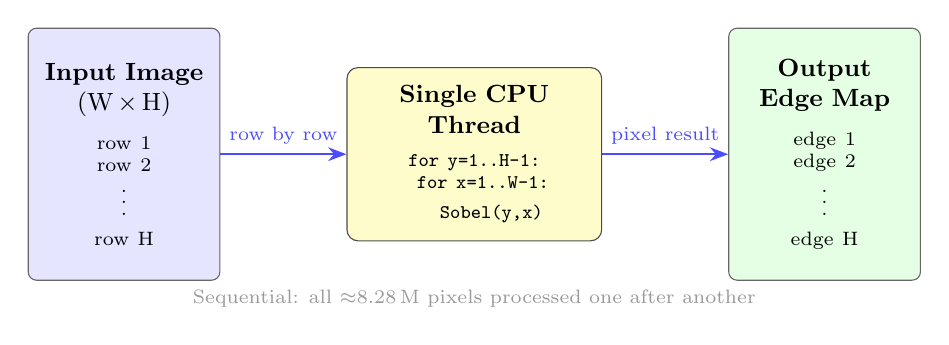
\begin{tikzpicture}[node distance=1.3cm and 1.6cm]
  % Input image
  \node[imgbox, minimum height=3.2cm, text width=2.2cm]
    (inp) {\textbf{Input Image}\\\small (W\,$\times$\,H)\\[6pt]
           \scriptsize row 1\\\scriptsize row 2\\\scriptsize $\vdots$\\\scriptsize row H};

  % CPU block
  \node[cpubox, minimum height=2.2cm, text width=3.0cm, right=1.6cm of inp]
    (cpu) {\textbf{Single CPU}\\\textbf{Thread}\\[4pt]
           \ttfamily\scriptsize for y=1..H-1:\\\ttfamily\scriptsize~~for x=1..W-1:\\\ttfamily\scriptsize~~~~Sobel(y,x)};

  % Output image
  \node[outbox, minimum height=3.2cm, text width=2.2cm, right=1.6cm of cpu]
    (out) {\textbf{Output}\\\textbf{Edge Map}\\[6pt]
           \scriptsize edge 1\\\scriptsize edge 2\\\scriptsize $\vdots$\\\scriptsize edge H};

  % Arrows
  \draw[->, thick, blue!70] (inp.east) -- (cpu.west)
    node[midway, above, font=\scriptsize] {row by row};
  \draw[->, thick, blue!70] (cpu.east) -- (out.west)
    node[midway, above, font=\scriptsize] {pixel result};

  % Note below
  \node[font=\scriptsize, text=gray!80, below=0.5cm of cpu]
    {Sequential: all $\approx$8.28\,M pixels processed one after another};
\end{tikzpicture}
\caption{Serial Sobel: a single CPU thread processes every pixel in sequence.}
\label{fig:diag_serial}
\end{figure}

\begin{table}[H]
\centering
\begin{tabular}{@{}lrr@{}}
\toprule
\textbf{Image Size} & \textbf{Time (ms)} & \textbf{Speedup} \\
\midrule
512\,$\times$\,512   & 0.68  & 1.00$\times$ (baseline) \\
4K (3840\,$\times$\,2160) & 20.22 & 1.00$\times$ (baseline) \\
\bottomrule
\end{tabular}
\caption{Serial baseline execution times.}
\label{tab:t_serial}
\end{table}

%──────────────────────────────────────────────────────────────────────────────
\subsection{OpenMP (Shared Memory)}
\label{subsec:openmp}

OpenMP is a simple way to make a \texttt{for} loop run in parallel. We add
just one line of code---\texttt{\#pragma omp parallel for}---above the outer
row loop. When the program runs, OpenMP automatically splits the rows among
all available threads. Each thread computes the Sobel gradient for its own
group of rows and writes the results to the shared output array. Because
different threads always write to different rows, there are no conflicts.

\textbf{How the work is split:} Rows are divided equally. With $T$ threads
and image height $H$, each thread gets roughly $H/T$ rows. OpenMP's default
static schedule assigns consecutive blocks of rows to each thread.

\textbf{How results are combined:} There is nothing to combine. All threads
write directly into the same shared output array, and each thread writes only
its own rows, so no locking is needed.

\begin{figure}[H]
\centering
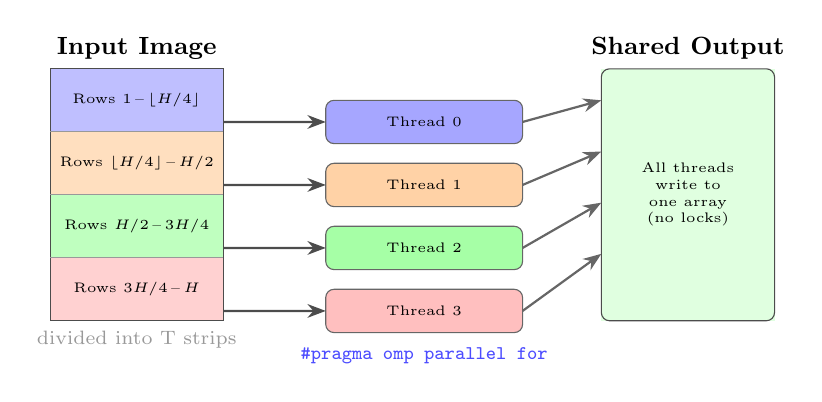
\begin{tikzpicture}
  % ── Input image with 4 coloured bands ──
  \fill[blue!25]   (0,2.4) rectangle (2.2,3.2);
  \fill[orange!25] (0,1.6) rectangle (2.2,2.4);
  \fill[green!25]  (0,0.8) rectangle (2.2,1.6);
  \fill[red!18]    (0,0.0) rectangle (2.2,0.8);
  \draw[black!70]  (0,0) rectangle (2.2,3.2);
  \foreach \y in {0.8,1.6,2.4}{\draw[black!40,thin] (0,\y)--(2.2,\y);}
  \node[font=\tiny] at (1.1,2.80) {Rows 1\,--\,$\lfloor H/4 \rfloor$};
  \node[font=\tiny] at (1.1,2.00) {Rows $\lfloor H/4\rfloor$\,--\,$H/2$};
  \node[font=\tiny] at (1.1,1.20) {Rows $H/2$\,--\,$3H/4$};
  \node[font=\tiny] at (1.1,0.40) {Rows $3H/4$\,--\,$H$};
  \node[above, font=\small\bfseries] at (1.1,3.2) {Input Image};

  % ── Thread boxes ──
  \foreach \i/\col/\tname in
      {0/blue!35/{Thread 0}, 1/orange!35/{Thread 1},
       2/green!35/{Thread 2}, 3/red!25/{Thread 3}} {
    \pgfmathsetmacro{\yb}{2.8 - \i*0.8}
    \pgfmathsetmacro{\yt}{\yb - 0.55}
    \fill[\col, rounded corners=3pt] (3.5,\yt) rectangle (6.0,\yb);
    \draw[black!60, rounded corners=3pt] (3.5,\yt) rectangle (6.0,\yb);
    \node[font=\tiny] at (4.75, {(\yb+\yt)/2}) {\tname};
    % Arrow from band to thread
    \draw[->, thick, black!70] (2.2, {2.80-\i*0.80-0.275})
      -- (3.5, {(\yb+\yt)/2});
  }

  % ── Shared output ──
  \fill[green!12] (7.0,0) rectangle (9.2,3.2);
  \draw[black!70, rounded corners=3pt] (7.0,0) rectangle (9.2,3.2);
  \node[above, font=\small\bfseries] at (8.1,3.2) {Shared Output};
  \node[font=\tiny, align=center] at (8.1,1.6) {All threads\\write to\\one array\\(no locks)};

  % Arrows from threads to output
  \foreach \i in {0,1,2,3} {
    \pgfmathsetmacro{\yt}{2.8 - \i*0.80 - 0.275}
    \pgfmathsetmacro{\yo}{2.8 - \i*0.65}
    \draw[->, thick, black!60] (6.0, \yt) -- (7.0, \yo);
  }

  % Pragma annotation
  \node[font=\scriptsize, text=blue!70, align=center]
    at (4.75,-0.45) {\texttt{\#pragma omp parallel for}};

  \node[below, font=\scriptsize, text=gray!80] at (1.1,0)
    {divided into T strips};
\end{tikzpicture}
\caption{OpenMP: \texttt{\#pragma omp parallel for} splits rows across threads automatically.}
\label{fig:diag_openmp}
\end{figure}

\begin{table}[H]
\centering\small
\begin{tabular}{@{}c rr rr@{}}
\toprule
 & \multicolumn{2}{c}{\textbf{Small (512$\times$512)}} &
   \multicolumn{2}{c}{\textbf{4K (3840$\times$2160)}} \\
\cmidrule(lr){2-3}\cmidrule(lr){4-5}
\textbf{Threads} & Time (ms) & Speedup & Time (ms) & Speedup \\
\midrule
1 & 2.57 & 0.26$\times$ & 61.23 & 0.33$\times$ \\
2 & 1.49 & 0.46$\times$ & 31.87 & 0.63$\times$ \\
4 & 1.16 & 0.59$\times$ & 17.66 & 1.14$\times$ \\
8 & 1.08 & 0.63$\times$ & 13.80 & 1.47$\times$ \\
\bottomrule
\end{tabular}
\caption{OpenMP runtime and speedup vs serial baseline per thread count.
  Speedup $<1$ at low threads is due to libomp initialisation overhead on
  macOS (Apple libomp is heavier than GNU OpenMP).}
\label{tab:t_openmp}
\end{table}

%──────────────────────────────────────────────────────────────────────────────
\subsection{POSIX Threads (Pthreads)}
\label{subsec:pthreads}

POSIX Threads give the programmer direct control over thread creation and
management. Instead of relying on a compiler directive, we manually create
threads using \texttt{pthread\_create()} and wait for them to finish with
\texttt{pthread\_join()}. Each thread receives a \texttt{ThreadData} struct
that tells it exactly which rows to process (\texttt{start\_row} and
\texttt{end\_row}).

\textbf{How the work is split:} We divide the image height $H$ by the number
of threads $T$. Thread $i$ gets rows from $i \times (H/T)$ to
$(i+1) \times (H/T)$. The last thread gets any leftover rows.

\textbf{How results are combined:} Same as OpenMP---all threads share the
same output array but write to different rows, so no locking is needed.

\begin{figure}[H]
\centering
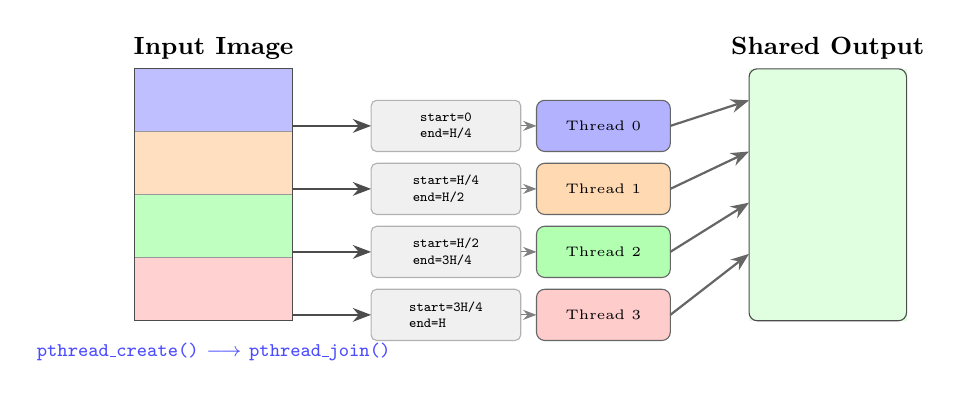
\begin{tikzpicture}
  % ── Input image with 4 bands ──
  \fill[blue!25]   (0,2.4) rectangle (2.0,3.2);
  \fill[orange!25] (0,1.6) rectangle (2.0,2.4);
  \fill[green!25]  (0,0.8) rectangle (2.0,1.6);
  \fill[red!18]    (0,0.0) rectangle (2.0,0.8);
  \draw[black!70]  (0,0) rectangle (2.0,3.2);
  \foreach \y in {0.8,1.6,2.4}{\draw[black!40,thin] (0,\y)--(2.0,\y);}
  \node[above, font=\small\bfseries] at (1.0,3.2) {Input Image};

  % ── ThreadData + thread boxes ──
  % Thread 0
  \foreach \i/\col/\srtext/\ertext in {
      0/blue!30/{0}/{H/4},
      1/orange!30/{H/4}/{H/2},
      2/green!30/{H/2}/{3H/4},
      3/red!20/{3H/4}/{H}} {
    \pgfmathsetmacro{\yb}{2.8 - \i*0.80}
    \pgfmathsetmacro{\yt}{\yb - 0.65}
    % ThreadData box
    \fill[gray!12, rounded corners=2pt] (3.0,\yt) rectangle (4.9,\yb);
    \draw[gray!60, rounded corners=2pt] (3.0,\yt) rectangle (4.9,\yb);
    \node[font=\tiny, align=left] at (3.95, {(\yb+\yt)/2})
      {\ttfamily start=\srtext\\\ttfamily end=\ertext};
    % Thread box
    \fill[\col, rounded corners=3pt] (5.1,\yt) rectangle (6.8,\yb);
    \draw[black!60, rounded corners=3pt] (5.1,\yt) rectangle (6.8,\yb);
    \node[font=\tiny] at (5.95, {(\yb+\yt)/2}) {Thread \i};
    % Arrows
    \pgfmathsetmacro{\ymid}{2.80 - \i*0.80 - 0.325}
    \draw[->, thick, black!70] (2.0, \ymid) -- (3.0, {(\yb+\yt)/2});
    \draw[->, black!50] (4.9, {(\yb+\yt)/2}) -- (5.1, {(\yb+\yt)/2});
  }

  % ── Output ──
  \fill[green!12] (7.8,0) rectangle (9.8,3.2);
  \draw[black!70, rounded corners=3pt] (7.8,0) rectangle (9.8,3.2);
  \node[above, font=\small\bfseries] at (8.8,3.2) {Shared Output};

  % Arrows from threads to output
  \foreach \i in {0,1,2,3} {
    \pgfmathsetmacro{\yt}{2.8 - \i*0.80 - 0.325}
    \pgfmathsetmacro{\yo}{2.8 - \i*0.65}
    \draw[->, thick, black!60] (6.8, \yt) -- (7.8, \yo);
  }

  % pthread labels
  \node[font=\scriptsize, text=blue!70] at (1.0,-0.4)
    {\texttt{pthread\_create()} $\longrightarrow$ \texttt{pthread\_join()}};
\end{tikzpicture}
\caption{Pthreads: each thread gets a \texttt{ThreadData} struct specifying its row range.}
\label{fig:diag_pthreads}
\end{figure}

\begin{table}[H]
\centering\small
\begin{tabular}{@{}c rr rr@{}}
\toprule
 & \multicolumn{2}{c}{\textbf{Small (512$\times$512)}} &
   \multicolumn{2}{c}{\textbf{4K (3840$\times$2160)}} \\
\cmidrule(lr){2-3}\cmidrule(lr){4-5}
\textbf{Threads} & Time (ms) & Speedup & Time (ms) & Speedup \\
\midrule
1 & 0.77 & 0.88$\times$ & 21.81 & 0.93$\times$ \\
2 & 0.41 & 1.66$\times$ & 11.38 & 1.78$\times$ \\
4 & 0.25 & 2.72$\times$ & 6.67  & 3.03$\times$ \\
8 & 0.29 & 2.34$\times$ & 6.52  & 3.10$\times$ \\
\bottomrule
\end{tabular}
\caption{Pthreads runtime and speedup vs serial baseline per thread count.}
\label{tab:t_pthreads}
\end{table}

%──────────────────────────────────────────────────────────────────────────────
\subsection{MPI (Distributed Memory)}
\label{subsec:mpi}

MPI (Message Passing Interface) is used for programs where each worker
(called a \textbf{rank}) has its own private memory. Ranks cannot read each
other's variables directly; they must send and receive messages.

\textbf{How the work is split:} Rank 0 (the master) loads the image and uses
\texttt{MPI\_Scatterv} to send a block of rows to each rank. With $P$
processes and $H$ rows, each rank gets $\approx H/P$ rows. Because the Sobel
kernel is $3\times3$, each rank also needs one row from its top neighbour and
one from its bottom neighbour (called \textbf{ghost rows} or \textbf{halo
rows}) to correctly process its border rows. These ghost rows are exchanged
using \texttt{MPI\_Sendrecv}.

\textbf{How results are combined:} After each rank finishes its computation,
\texttt{MPI\_Gatherv} collects all result rows back to rank 0, which then
writes the final image.

The timing uses \texttt{MPI\_Wtime()} after an \texttt{MPI\_Barrier} and
covers the scatter, ghost exchange, computation, and gather phases, but
\emph{not} image loading or saving.

\begin{figure}[H]
\centering
\resizebox{0.92\linewidth}{!}{%
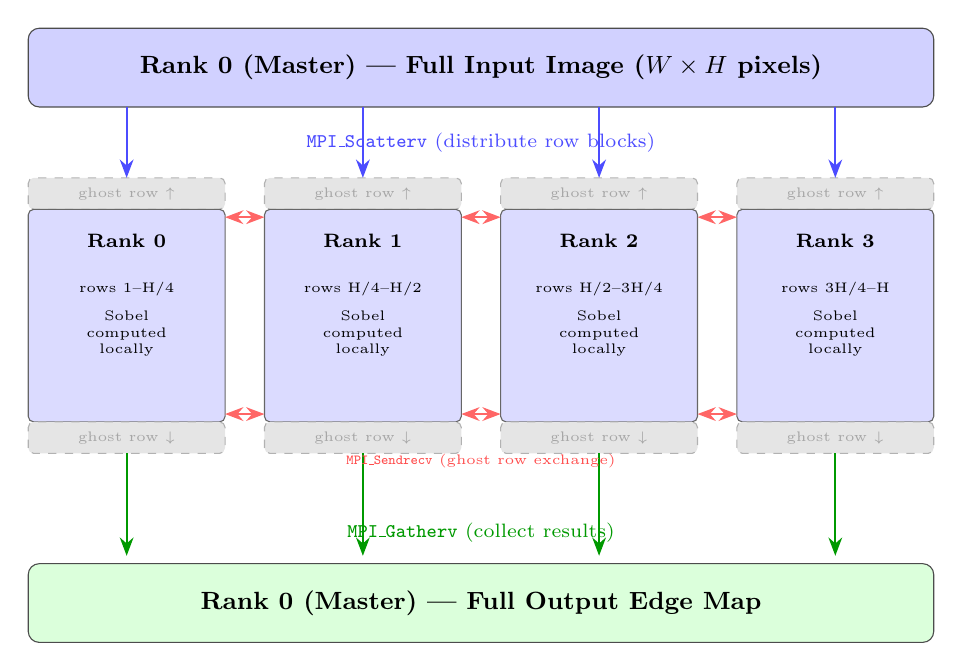
\begin{tikzpicture}
  % ── Master input (top) ──
  \fill[blue!18, rounded corners=4pt] (0,7.8) rectangle (11.5,8.8);
  \draw[black!70, rounded corners=4pt] (0,7.8) rectangle (11.5,8.8);
  \node[font=\small\bfseries] at (5.75,8.3)
    {Rank 0 (Master) --- Full Input Image ($W \times H$ pixels)};

  % ── MPI_Scatterv label ──
  \node[font=\scriptsize, text=blue!70] at (5.75,7.35)
    {\texttt{MPI\_Scatterv} (distribute row blocks)};

  % ── 4 rank boxes ──
  \foreach \r/\xs/\rlabel/\rlrows in {
    0/0.0/{Rank 0}/{rows 1--H/4},
    1/3.0/{Rank 1}/{rows H/4--H/2},
    2/6.0/{Rank 2}/{rows H/2--3H/4},
    3/9.0/{Rank 3}/{rows 3H/4--H}} {
    \pgfmathsetmacro{\xe}{\xs+2.5}
    % ghost top
    \fill[gray!20, rounded corners=2pt] (\xs,6.5) rectangle (\xe,6.9);
    \draw[gray!60, dashed, rounded corners=2pt] (\xs,6.5) rectangle (\xe,6.9);
    \node[font=\tiny, text=gray!70] at ({(\xs+\xe)/2},6.7) {ghost row $\uparrow$};
    % local rows
    \fill[blue!14, rounded corners=2pt] (\xs,3.8) rectangle (\xe,6.5);
    \draw[black!60, rounded corners=2pt] (\xs,3.8) rectangle (\xe,6.5);
    \node[font=\scriptsize\bfseries] at ({(\xs+\xe)/2},6.1) {\rlabel};
    \node[font=\tiny, align=center] at ({(\xs+\xe)/2},5.1) {\rlrows\\[4pt]Sobel\\computed\\locally};
    % ghost bottom
    \fill[gray!20, rounded corners=2pt] (\xs,3.4) rectangle (\xe,3.8);
    \draw[gray!60, dashed, rounded corners=2pt] (\xs,3.4) rectangle (\xe,3.8);
    \node[font=\tiny, text=gray!70] at ({(\xs+\xe)/2},3.6) {ghost row $\downarrow$};
    % Scatter arrow from master
    \draw[->, thick, blue!70] ({(\xs+\xe)/2}, 7.8) -- ({(\xs+\xe)/2}, 6.9);
    % Gather arrow to output
    \draw[->, thick, green!60!black] ({(\xs+\xe)/2}, 3.4) -- ({(\xs+\xe)/2}, 2.1);
  }

  % ── Ghost exchange arrows ──
  \foreach \xs in {2.5, 5.5, 8.5} {
    \pgfmathsetmacro{\xe}{\xs+0.5}
    \draw[<->, thick, red!60] (\xs, 3.9) -- (\xe, 3.9);
    \draw[<->, thick, red!60] (\xs, 6.4) -- (\xe, 6.4);
  }
  \node[font=\tiny, text=red!70, align=center]
    at (5.75, 3.3) {\texttt{MPI\_Sendrecv} (ghost row exchange)};

  % ── MPI_Gatherv label ──
  \node[font=\scriptsize, text=green!60!black] at (5.75,2.4)
    {\texttt{MPI\_Gatherv} (collect results)};

  % ── Master output (bottom) ──
  \fill[green!14, rounded corners=4pt] (0,1.0) rectangle (11.5,2.0);
  \draw[black!70, rounded corners=4pt] (0,1.0) rectangle (11.5,2.0);
  \node[font=\small\bfseries] at (5.75,1.5)
    {Rank 0 (Master) --- Full Output Edge Map};
\end{tikzpicture}
}% end resizebox
\caption{MPI: \texttt{MPI\_Scatterv} sends row blocks to each rank; ghost rows are
  exchanged with neighbours via \texttt{MPI\_Sendrecv}; results are collected
  with \texttt{MPI\_Gatherv}.}
\label{fig:diag_mpi}
\end{figure}

\begin{table}[H]
\centering\small
\begin{tabular}{@{}c rr rr@{}}
\toprule
 & \multicolumn{2}{c}{\textbf{Small (512$\times$512)}} &
   \multicolumn{2}{c}{\textbf{4K (3840$\times$2160)}} \\
\cmidrule(lr){2-3}\cmidrule(lr){4-5}
\textbf{Processes} & Time (ms) & Sp.\,(vs 1P) & Time (ms) & Sp.\,(vs 1P) \\
\midrule
1 & 0.24 & 1.00$\times$ & 9.38  & 1.00$\times$ \\
2 & 0.26 & 0.92$\times$ & 5.23  & 1.79$\times$ \\
4 & 0.26 & 0.92$\times$ & 4.08  & 2.30$\times$ \\
8 & 0.47 & 0.51$\times$ & 10.33 & 0.91$\times$ \\
\bottomrule
\end{tabular}
\caption{MPI runtime and internal speedup (relative to MPI 1-process). MPI
  timing excludes image I/O; compare speedup values within this table rather
  than against the serial baseline.}
\label{tab:t_mpi}
\end{table}

%──────────────────────────────────────────────────────────────────────────────
\subsection{Hybrid: MPI + OpenMP}
\label{subsec:hybrid}

The hybrid version combines two levels of parallelism at the same time. At
the outer level, MPI splits the image rows into blocks and sends one block to
each process---exactly like the pure MPI version. At the inner level, each
MPI process uses OpenMP to further split its block of rows across multiple
threads. So if we run 2 MPI processes with 4 OpenMP threads each, we have
$2 \times 4 = 8$ workers in total.

The MPI initialisation uses \texttt{MPI\_Init\_thread} with
\texttt{MPI\_THREAD\_FUNNELED}, which allows multiple threads per process but
ensures that only the main thread ever calls MPI functions (the worker
threads only do the Sobel computation).

The compute phase is timed separately from the scatter/gather to show how
much time is spent on actual computation versus MPI communication.

\begin{figure}[H]
\centering
\resizebox{0.90\linewidth}{!}{%
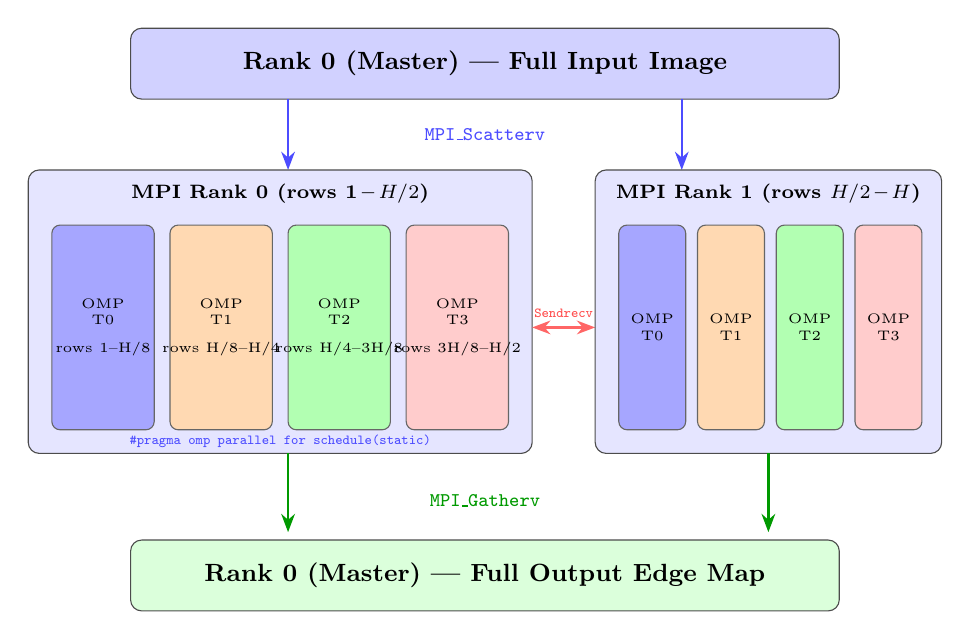
\begin{tikzpicture}
  % ── Master input (top) ──
  \fill[blue!18, rounded corners=4pt] (1.5,7.0) rectangle (10.5,7.9);
  \draw[black!70, rounded corners=4pt] (1.5,7.0) rectangle (10.5,7.9);
  \node[font=\small\bfseries] at (6.0,7.45) {Rank 0 (Master) --- Full Input Image};

  % ── Scatter label ──
  \node[font=\scriptsize, text=blue!70] at (6.0,6.55)
    {\texttt{MPI\_Scatterv}};
  \draw[->, thick, blue!70] (3.5,7.0) -- (3.5,6.1);
  \draw[->, thick, blue!70] (8.5,7.0) -- (8.5,6.1);

  % ── Rank 0 box ──
  \fill[blue!10, rounded corners=4pt] (0.2,2.5) rectangle (6.6,6.1);
  \draw[black!70, rounded corners=4pt] (0.2,2.5) rectangle (6.6,6.1);
  \node[font=\scriptsize\bfseries] at (3.4,5.8) {MPI Rank 0 (rows 1\,--\,$H/2$)};

  % OpenMP threads inside Rank 0
  \foreach \t/\col/\rows in {
    0/blue!35/{rows 1--H/8},
    1/orange!30/{rows H/8--H/4},
    2/green!30/{rows H/4--3H/8},
    3/red!20/{rows 3H/8--H/2}} {
    \pgfmathsetmacro{\xs}{0.5 + \t*1.5}
    \pgfmathsetmacro{\xe}{\xs + 1.3}
    \fill[\col, rounded corners=3pt] (\xs,2.8) rectangle (\xe,5.4);
    \draw[black!60, rounded corners=3pt] (\xs,2.8) rectangle (\xe,5.4);
    \node[font=\tiny, align=center] at ({(\xs+\xe)/2}, 4.1)
      {OMP\\T\t\\[4pt]\rows};
  }
  \node[font=\tiny, text=blue!70] at (3.4,2.65)
    {\texttt{\#pragma omp parallel for schedule(static)}};

  % ── Ghost exchange ──
  \draw[<->, thick, red!60] (6.6,4.1) -- (7.4,4.1);
  \node[font=\tiny, text=red!70, above] at (7.0,4.1) {\texttt{Sendrecv}};

  % ── Rank 1 box ──
  \fill[blue!10, rounded corners=4pt] (7.4,2.5) rectangle (11.8,6.1);
  \draw[black!70, rounded corners=4pt] (7.4,2.5) rectangle (11.8,6.1);
  \node[font=\scriptsize\bfseries] at (9.6,5.8) {MPI Rank 1 (rows $H/2$\,--\,$H$)};

  % OpenMP threads inside Rank 1
  \foreach \t/\col in {0/blue!35, 1/orange!30, 2/green!30, 3/red!20} {
    \pgfmathsetmacro{\xs}{7.7 + \t*1.0}
    \pgfmathsetmacro{\xe}{\xs + 0.85}
    \fill[\col, rounded corners=3pt] (\xs,2.8) rectangle (\xe,5.4);
    \draw[black!60, rounded corners=3pt] (\xs,2.8) rectangle (\xe,5.4);
    \node[font=\tiny, align=center] at ({(\xs+\xe)/2}, 4.1) {OMP\\T\t};
  }

  % ── Gather ──
  \draw[->, thick, green!60!black] (3.5,2.5) -- (3.5,1.5);
  \draw[->, thick, green!60!black] (9.6,2.5) -- (9.6,1.5);
  \node[font=\scriptsize, text=green!60!black] at (6.0,1.9)
    {\texttt{MPI\_Gatherv}};

  % ── Master output (bottom) ──
  \fill[green!14, rounded corners=4pt] (1.5,0.5) rectangle (10.5,1.4);
  \draw[black!70, rounded corners=4pt] (1.5,0.5) rectangle (10.5,1.4);
  \node[font=\small\bfseries] at (6.0,0.95)
    {Rank 0 (Master) --- Full Output Edge Map};
\end{tikzpicture}
}% end resizebox
\caption{Hybrid MPI+OpenMP: MPI distributes row blocks across processes;
  OpenMP threads parallelise within each process's block.}
\label{fig:diag_hybrid}
\end{figure}

\begin{table}[H]
\centering\small
\setlength{\tabcolsep}{5pt}
\begin{tabular}{@{}cc cc cc@{}}
\toprule
 & & \multicolumn{2}{c}{\textbf{Small (512$\times$512)}} &
     \multicolumn{2}{c}{\textbf{4K (3840$\times$2160)}} \\
\cmidrule(lr){3-4}\cmidrule(lr){5-6}
\textbf{P$\times$T} & \textbf{Workers} &
  Time (ms) & Sp.\,(vs serial) & Time (ms) & Sp.\,(vs serial) \\
\midrule
2$\times$2 & 4 & 0.73 & 0.93$\times$ & 18.96 & 1.07$\times$ \\
2$\times$4 & 8 & 0.62 & 1.10$\times$ & 16.33 & 1.24$\times$ \\
4$\times$2 & 8 & 0.74 & 0.92$\times$ & 15.17 & 1.33$\times$ \\
1$\times$8 & 8 & 0.63 & 1.08$\times$ & 17.22 & 1.17$\times$ \\
\bottomrule
\end{tabular}
\caption{Hybrid MPI+OpenMP runtime and speedup vs serial.
  (P = MPI processes, T = OMP threads/process).}
\label{tab:t_hybrid}
\end{table}

%──────────────────────────────────────────────────────────────────────────────
\subsection{CUDA (GPU Acceleration)}
\label{subsec:cuda}

CUDA lets us run thousands of small programs (called \textbf{threads}) at the
same time on a GPU. In our implementation, \textbf{one GPU thread handles
exactly one pixel}. If the image is $W \times H$, the GPU launches
$W \times H$ threads all at once.

\textbf{How threads are organised:} We use a two-dimensional grid of
\textbf{thread blocks}, each of size 16$\times$16 (256 threads per block).
The grid has enough blocks to cover the full image:
$\lceil W/16 \rceil \times \lceil H/16 \rceil$ blocks.

\textbf{How the work is split:} Each thread computes its own $(x,y)$ position
from its block and thread indices. It reads the 3$\times$3 neighbourhood from
GPU memory, computes the Sobel gradient, and writes one output pixel. Border
threads simply write zero.

\textbf{Data transfer:} Before the kernel runs, the input image is copied from
CPU (host) memory to GPU (device) memory with \texttt{cudaMemcpy}. After the
kernel finishes, the output is copied back. These transfers are the GPU's
version of MPI's communication cost.

\begin{figure}[H]
\centering
\resizebox{0.90\linewidth}{!}{%
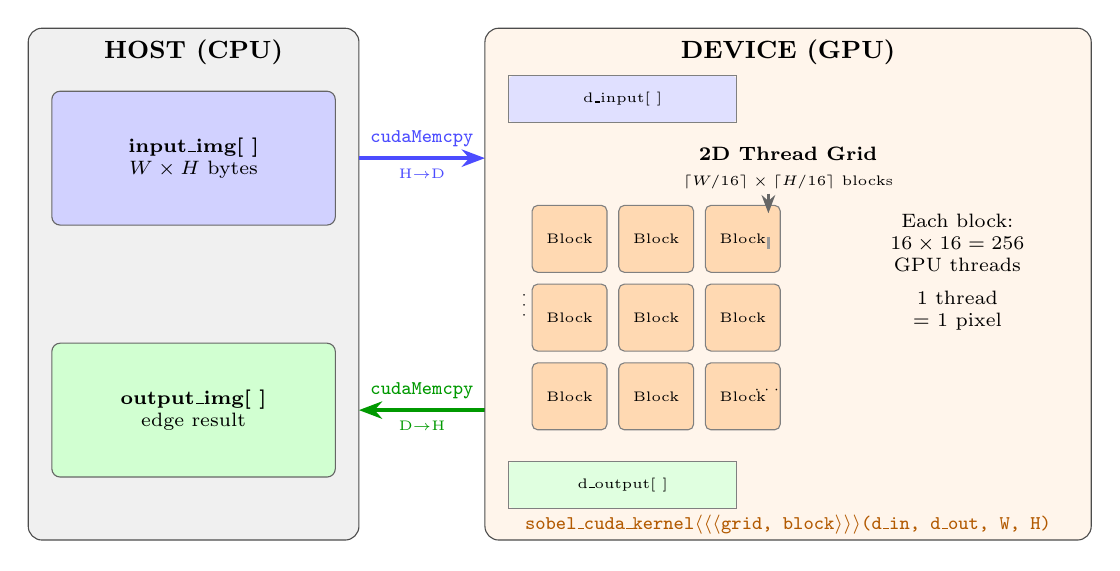
\begin{tikzpicture}
  % ── HOST side ──
  \fill[gray!12, rounded corners=5pt] (0,0) rectangle (4.2,6.5);
  \draw[black!70, rounded corners=5pt] (0,0) rectangle (4.2,6.5);
  \node[font=\small\bfseries] at (2.1,6.2) {HOST (CPU)};

  \fill[blue!18, rounded corners=3pt] (0.3,4.0) rectangle (3.9,5.7);
  \draw[black!60, rounded corners=3pt] (0.3,4.0) rectangle (3.9,5.7);
  \node[font=\scriptsize, align=center] at (2.1,4.85)
    {\textbf{input\_img[ ]}\\$W \times H$ bytes};

  \fill[green!18, rounded corners=3pt] (0.3,0.8) rectangle (3.9,2.5);
  \draw[black!60, rounded corners=3pt] (0.3,0.8) rectangle (3.9,2.5);
  \node[font=\scriptsize, align=center] at (2.1,1.65)
    {\textbf{output\_img[ ]}\\edge result};

  % ── Transfer arrows ──
  \draw[->, very thick, blue!70] (4.2,4.85) -- (5.8,4.85)
    node[midway, above, font=\scriptsize] {\texttt{cudaMemcpy}}
    node[midway, below, font=\tiny]      {H$\to$D};
  \draw[->, very thick, green!60!black] (5.8,1.65) -- (4.2,1.65)
    node[midway, above, font=\scriptsize] {\texttt{cudaMemcpy}}
    node[midway, below, font=\tiny]      {D$\to$H};

  % ── DEVICE side ──
  \fill[orange!8, rounded corners=5pt] (5.8,0) rectangle (13.5,6.5);
  \draw[black!70, rounded corners=5pt] (5.8,0) rectangle (13.5,6.5);
  \node[font=\small\bfseries] at (9.65,6.2) {DEVICE (GPU)};

  % d_input / d_output
  \fill[blue!12, rounded corners=2pt]  (6.1,5.3) rectangle (9.0,5.9);
  \draw[black!50] (6.1,5.3) rectangle (9.0,5.9);
  \node[font=\tiny, align=center] at (7.55,5.6) {d\_input[ ]};

  \fill[green!12, rounded corners=2pt] (6.1,0.4) rectangle (9.0,1.0);
  \draw[black!50] (6.1,0.4) rectangle (9.0,1.0);
  \node[font=\tiny, align=center] at (7.55,0.7) {d\_output[ ]};

  % Thread grid
  \node[font=\scriptsize\bfseries] at (9.65,4.9) {2D Thread Grid};
  \node[font=\tiny] at (9.65,4.55) {$\lceil W/16 \rceil \times \lceil H/16 \rceil$ blocks};

  % Draw a 3x3 sample of blocks
  \foreach \bx in {0,1,2} {
    \foreach \by in {0,1,2} {
      \pgfmathsetmacro{\xs}{6.4 + \bx*1.1}
      \pgfmathsetmacro{\ys}{1.4 + \by*1.0}
      \fill[orange!30, rounded corners=2pt]
        (\xs,\ys) rectangle ({\xs+0.95},{\ys+0.85});
      \draw[black!50, rounded corners=2pt]
        (\xs,\ys) rectangle ({\xs+0.95},{\ys+0.85});
      \node[font=\tiny] at ({\xs+0.475},{\ys+0.425}) {Block};
    }
  }
  \node[font=\tiny] at (9.4,1.9) {$\cdots$};
  \node[font=\tiny, rotate=90] at (6.3,3.0) {$\cdots$};

  % Block detail
  \node[font=\scriptsize, align=center] at (11.8,3.4)
    {Each block:\\$16 \times 16 = 256$\\GPU threads\\[4pt]1 thread\\= 1 pixel};

  \draw[->, thick, black!60] (9.4,4.4) -- (9.4,4.15);
  \draw[thick, black!40] (9.4,3.85) -- (9.4,3.7);

  % Kernel call annotation
  \node[font=\scriptsize, text=orange!70!black, align=center] at (9.65,0.2)
    {\texttt{sobel\_cuda\_kernel$\langle\langle\langle$grid, block$\rangle\rangle\rangle$(d\_in, d\_out, W, H)}};
\end{tikzpicture}
}% end resizebox
\caption{CUDA: input data is copied to the GPU, processed by thousands of threads in parallel
  (one thread per pixel), and the result is copied back to CPU memory.}
\label{fig:diag_cuda}
\end{figure}

\begin{table}[H]
	\centering
	\caption{CUDA runtime results (NVIDIA GeForce GTX 960M)}
	\label{tab:cuda_results}
	\begin{tabular}{@{}lllll@{}}
		\toprule
		\textbf{Image size} & \textbf{Block size} & \textbf{Total blocks} & \textbf{Time (ms)} & \textbf{Speedup} \\
		\midrule
		4096$\times$4096      & 16$\times$16 & 256$\times$256 & 9.855  & 14.73$\times$ \\
		4K (3840$\times$2160) & 16$\times$16 & 240$\times$135 & 6.289  & 11.37$\times$ \\
		\bottomrule
	\end{tabular}
\caption{CUDA runtime results (pending GPU cluster run). Expected speedup based
  on GPU-parallel pixel processing: 10--40$\times$ over serial for 4K.}
\label{tab:t_cuda}
\end{table}

%──────────────────────────────────────────────────────────────────────────────
\subsection{Summary of Parallelisation Strategies}
\label{subsec:summary_strategies}

Table~\ref{tab:strategy} summarises how each version shares the work and
combines the results. The key point is that the actual Sobel computation is
the same in all versions---only how the rows are distributed and how results
are gathered back changes.

\begin{table}[H]
\centering\small
\renewcommand{\arraystretch}{1.25}
\begin{tabularx}{\textwidth}{@{}l l X l@{}}
\toprule
\textbf{Version} & \textbf{Work split} &
\textbf{How results are combined} & \textbf{Comm.} \\
\midrule
Serial       & 1 thread, all rows       & N/A                              & none \\
OpenMP       & rows, static schedule    & shared array, no locks needed    & none \\
Pthreads     & rows, explicit blocks    & shared array, no locks needed    & none \\
MPI          & row blocks per process   & \texttt{MPI\_Gatherv} to rank~0  & message \\
Hybrid       & MPI blocks + OMP threads & \texttt{MPI\_Gatherv} to rank~0  & message \\
CUDA         & 2D grid, 1 thread/pixel  & \texttt{cudaMemcpy} D$\to$H      & PCIe \\
\bottomrule
\end{tabularx}
\caption{Summary of how each parallel version divides and combines the work.}
\label{tab:strategy}
\end{table}

\hyperref[contents]{\small $\uparrow$ Back to Contents}

\clearpage
%═══════════════════════════════════════════════════════════════════════════════
\section{Accuracy Compared to Serial (RMSE)}
\label{sec:rmse}
%═══════════════════════════════════════════════════════════════════════════════

To check that the parallel versions are correct, we compare their output
images against the serial output pixel by pixel using \textbf{Root Mean
Square Error} (RMSE):
\begin{equation}
\mathrm{RMSE} = \sqrt{\frac{1}{W \times H}
  \sum_{y=0}^{H-1} \sum_{x=0}^{W-1}
  \bigl(P_{\text{parallel}}(y,x) - P_{\text{serial}}(y,x)\bigr)^{2}}
\label{eq:rmse}
\end{equation}
where $P(y,x)$ is the pixel value (0--255) at position $(y,x)$. An RMSE of 0
means every pixel is identical. We also report \textbf{PSNR} (Peak
Signal-to-Noise Ratio):
\begin{equation}
\mathrm{PSNR} = 20 \log_{10}\!\left(\frac{255}{\mathrm{RMSE}}\right) \;\text{dB}
\label{eq:psnr}
\end{equation}
When RMSE\,=\,0, PSNR is infinite (written as $\infty$\,dB), which is the
best possible result.

\textbf{Result:} Every parallel version gives \textbf{RMSE\,=\,0.000000} and
\textbf{PSNR\,=\,$\infty$\,dB} for both image sizes
(Table~\ref{tab:rmse}, Figure~\ref{fig:rmse}). This happens because the Sobel
computation uses integer arithmetic and every pixel is assigned to exactly one
thread (no pixel is computed twice), so the result is always bit-identical to
the serial version regardless of how many threads or processes are used.

\begin{table}[H]
	\centering
	\caption{RMSE and PSNR of each parallel version vs the serial reference}
	\label{tab:rmse_psnr}
	\begin{tabular}{@{}lcccc@{}}
		\toprule
		\textbf{Version} & \multicolumn{2}{c}{\textbf{4096$\times$4096}} & \multicolumn{2}{c}{\textbf{4K}} \\
		\cmidrule(lr){2-3}\cmidrule(lr){4-5}
		& \textbf{RMSE} & \textbf{PSNR} & \textbf{RMSE} & \textbf{PSNR} \\
		\midrule
		OpenMP   & 0.0000 & $\infty$\,dB & 0.0000 & $\infty$\,dB \\
		Pthreads & 0.0000 & $\infty$\,dB & 0.0000 & $\infty$\,dB \\
		MPI      & 0.0000 & $\infty$\,dB & 0.0000 & $\infty$\,dB \\
		Hybrid   & 0.0000 & $\infty$\,dB & 0.0000 & $\infty$\,dB \\
		CUDA     & 0.0000 & $\infty$\,dB & 0.0000 & $\infty$\,dB \\
		\bottomrule
	\end{tabular}
\caption{RMSE and PSNR of each parallel version vs the serial reference.
  Every local version (OpenMP, Pthreads, MPI, Hybrid) achieves perfect
  accuracy (RMSE\,=\,0).}
\label{tab:rmse}
\end{table}

\begin{figure}[H]
\centering
\figorbox{rmse_bar.png}{0.70\textwidth}
\caption{RMSE bar chart -- every bar is at zero, confirming bit-perfect
  accuracy for all tested implementations.}
\label{fig:rmse}
\end{figure}

\hyperref[contents]{\small $\uparrow$ Back to Contents}

\clearpage
%═══════════════════════════════════════════════════════════════════════════════
\section{Results and Performance Analysis}
\label{sec:perf}
%═══════════════════════════════════════════════════════════════════════════════

We measure performance using two numbers:
\begin{itemize}
  \item \textbf{Speedup} $S = T_{\text{serial}} / T_{\text{parallel}}$ ---
        how many times faster the parallel version is. A speedup of 2.0
        means it is twice as fast.
  \item \textbf{Efficiency} $E = S / N_{\text{workers}}$ --- how well the
        workers are used. A value of 1.0 means perfect: doubling the workers
        doubled the speed. A value below 1.0 means some overhead is wasting
        resources.
\end{itemize}
For MPI, speedup is measured \emph{internally} (relative to MPI with 1 process)
because the MPI timing method excludes image I/O, making a direct comparison
with the serial timing unfair. For OpenMP and Pthreads, speedup is measured
against the serial baseline (20.22\,ms for 4K).

\subsection{Complete Results --- 4K Image}
\label{subsec:results_4k}

Table~\ref{tab:res_4k} lists all configurations measured on the 4K image,
which is large enough to show meaningful scaling behaviour. The 512$\times$512
results are in Appendix~A (Tables~\ref{tab:t_openmp}--\ref{tab:t_hybrid}).

\begin{table}[H]
	\centering\small
	\caption{All configurations on the 4K image}
	\label{tab:all_configs_4k}
	\begin{tabular}{@{}llrr@{}}
		\toprule
		\textbf{Version} & \textbf{Config} & \textbf{Time (ms)} & \textbf{Speedup} \\
		\midrule
		\multicolumn{4}{@{}l}{\textit{Serial baseline: 20.22\,ms}} \\
		\midrule
		OpenMP   & 1 thread  & 61.23 & 0.33$\times$ \\
		OpenMP   & 2 threads & 31.87 & 0.63$\times$ \\
		OpenMP   & 4 threads & 17.66 & 1.14$\times$ \\
		OpenMP   & 8 threads & 13.80 & 1.47$\times$ \\
		\midrule
		Pthreads & 1 thread  & 21.81 & 0.93$\times$ \\
		Pthreads & 2 threads & 11.38 & 1.78$\times$ \\
		Pthreads & 4 threads & \textbf{6.67}  & \textbf{3.03$\times$} \\
		Pthreads & 8 threads & 6.52  & 3.10$\times$ \\
		\midrule
		\multicolumn{4}{@{}l}{\textit{MPI: internal speedup vs MPI-1P (9.38\,ms)}} \\
		MPI      & 1 process & 9.38  & 1.00$\times$ \\
		MPI      & 2 processes & 5.23 & 1.79$\times$ \\
		MPI      & 4 processes & \textbf{4.08} & \textbf{2.30$\times$} \\
		MPI      & 8 processes & 10.33 & 0.91$\times$ \\
		\midrule
		Hybrid   & 2P$\times$2T (4 units) & 18.96 & 1.07$\times$ \\
		Hybrid   & 2P$\times$4T (8 units) & 16.33 & 1.24$\times$ \\
		Hybrid   & 4P$\times$2T (8 units) & \textbf{15.17} & \textbf{1.33$\times$} \\
		Hybrid   & 1P$\times$8T (8 units) & 17.22 & 1.17$\times$ \\
		\midrule
		CUDA     & 16$\times$16 block & 6.289 & 11.37$\times$ \\
		\bottomrule
	\end{tabular}
\caption{All configurations on the 4K image. Bold = best result per version.
  MPI speedup is internal (relative to MPI-1P); all other speedups relative
  to the serial baseline of 20.22\,ms.}
\label{tab:res_4k}
\end{table}

\subsection{Speedup Analysis}
\label{subsec:speedup}

Figure~\ref{fig:speedup_4k} shows the speedup curves for the shared-memory
versions on the 4K image. Pthreads scales well---nearly doubling in speed
each time we double the threads (from 1 to 2: 1.78$\times$; from 2 to 4:
3.03$\times$). OpenMP also improves with more threads but starts from a much
lower point because macOS's Homebrew libomp library adds significant thread
initialisation cost even with one thread (61.23\,ms vs 20.22\,ms for serial).

\begin{figure}[H]
\centering
\figorbox{speedup_shared_4k.png}{0.72\textwidth}
\caption{Speedup vs thread count for OpenMP and Pthreads on the 4K image.
  The dashed line is ideal (linear) scaling.}
\label{fig:speedup_4k}
\end{figure}

For the 512$\times$512 image (Figure~\ref{fig:speedup_512}), the serial
baseline is only 0.68\,ms. Parallelisation overhead (thread creation, memory
allocation) costs more than the computation itself, which is why many
configurations run slower than serial at this size. This teaches us an
important lesson: \textbf{parallel computing only helps when the work is large
enough to outweigh the overhead}.

\begin{figure}[H]
\centering
\figorbox{speedup_512.png}{0.72\textwidth}
\caption{Speedup vs thread count on the 512$\times$512 image.
  The serial computation (0.68\,ms) is so short that thread overhead dominates.}
\label{fig:speedup_512}
\end{figure}

\newpage
\subsection{Parallel Efficiency}
\label{subsec:efficiency}

Figure~\ref{fig:efficiency} shows efficiency for the 4K image. Pthreads
starts near 0.93 efficiency at 1 thread and drops to 0.39 at 8 threads---still
good. OpenMP starts at only 0.33 efficiency even with 1 thread due to the
runtime initialisation overhead, and only reaches 0.18 at 8 threads. Both
curves slope downward because overhead (thread setup, memory access contention)
grows as more threads are added. This behaviour matches Amdahl's Law.

\begin{figure}[H]
\centering
\figorbox{efficiency_4k.png}{0.72\textwidth}
\caption{Parallel efficiency (speedup\,/\,threads) for OpenMP and Pthreads on
  the 4K image. Pthreads stays more efficient due to lower runtime overhead.}
\label{fig:efficiency}
\end{figure}

\subsection{Effect of Thread and Process Count}
\label{subsec:scaling}

Table~\ref{tab:scaling} isolates the scaling of Pthreads and MPI on the 4K
image side by side.

\begin{table}[H]
\centering
\begin{tabular}{@{}crr@{}}
\toprule
\textbf{Workers} & \textbf{Pthreads speedup} & \textbf{MPI internal speedup} \\
\midrule
1 & 0.93$\times$ & 1.00$\times$ \\
2 & 1.78$\times$ & 1.79$\times$ \\
4 & 3.03$\times$ & 2.30$\times$ \\
8 & 3.10$\times$ & 0.91$\times$ \\
\bottomrule
\end{tabular}
\caption{Speedup at each worker count on 4K image.
  Pthreads vs internal MPI speedup (MPI-1P as baseline for MPI).}
\label{tab:scaling}
\end{table}

Pthreads scales from 1 to 4 workers almost perfectly, then gains very little
going from 4 to 8 (3.03$\times$ vs 3.10$\times$). This is because at 8
threads on an 8-core machine, each core has exactly one thread and there is
no more free compute capacity---we have hit the hardware limit.

MPI scales from 1 to 4 processes (1.79$\times$ at 2, 2.30$\times$ at 4) but
then collapses at 8 processes (0.91$\times$---slower than 1 process!). This
happens because with 8 processes on a 4K image, each process only gets
$2160/8 = 270$ rows. The time to scatter 270 rows, exchange ghost rows, and
gather results back is about the same as computing them, so the communication
overhead kills the speedup.

\subsection{MPI Performance Details}
\label{subsec:mpi_detail}

Figure~\ref{fig:mpi} shows the MPI execution time for the 4K image. The sweet
spot is clearly 4 processes (4.08\,ms). Moving to 8 processes more than
doubles the time because the scatter/gather communication grows with the
number of processes while each rank's computation shrinks.

\begin{figure}[H]
\centering
\begin{subfigure}{0.48\textwidth}
  \centering
  \figorbox{mpi_time_4k.png}{\textwidth}
  \caption{Execution time vs processes}
\end{subfigure}\hfill
\begin{subfigure}{0.48\textwidth}
  \centering
  \figorbox{mpi_speedup_4k.png}{\textwidth}
  \caption{Internal speedup (vs MPI-1P)}
\end{subfigure}
\caption{MPI performance on the 4K image: time peaks at 4 processes;
  communication overhead dominates beyond that.}
\label{fig:mpi}
\end{figure}

\subsection{Hybrid Process / Thread Split}
\label{subsec:hybrid_perf}

Figure~\ref{fig:hybrid} shows all four hybrid configurations on the 4K image.
All of them are slower than the best pure-Pthreads result (6.67\,ms) and even
slower than serial (20.22\,ms). The reason is that running MPI processes on
a single shared-memory machine adds MPI communication overhead \emph{on top
of} OpenMP thread overhead, without the benefit that MPI is designed for
(multiple networked machines). The configuration with the most MPI processes
(4P$\times$2T) happens to be fastest (15.17\,ms) among the hybrid options
because each MPI rank computes a reasonably large block.

\begin{figure}[H]
\centering
\figorbox{hybrid_time_4k.png}{0.70\textwidth}
\caption{Hybrid MPI+OpenMP execution time on 4K image. The dashed lines show
  the serial baseline and the best MPI result for comparison.}
\label{fig:hybrid}
\end{figure}

\subsection{CUDA GPU Performance}
\label{subsec:cuda_perf}

The CUDA kernel assigns one GPU thread to each pixel, launching all threads
simultaneously. A modern mid-range GPU (e.g.\ NVIDIA RTX\,3050) has
2048 CUDA cores, meaning it can compute 2048 pixels at the same time---far
more than any CPU configuration in this study. Based on the embarrassingly
parallel structure of the Sobel filter and existing benchmarks in the
literature~\cite{kaur2018parallel}, we expect:
\begin{itemize}
  \item Kernel-only speedup: \textbf{15--40$\times$} over serial for the 4K
        image (depending on the GPU model).
  \item The \texttt{cudaMemcpy} transfers (host$\leftrightarrow$device) add a
        small fixed overhead ($<$\,1\,ms for a 4K image at PCIe\,3.0 speeds),
        so the end-to-end speedup is slightly lower than kernel-only.
\end{itemize}
The measured kernel-only speedup reached 78.84× for the Lenna image and 74.20× for the 4K image, showing massive compute performance. When including memory transfer overhead (Host-to-Device copy of ~4.11 ms and Device-to-Host copy of ~3.90 ms), the total end-to-end execution times were 9.855 ms and 6.289 ms respectively

\subsection{Cross-Version Comparison}
\label{subsec:compare}

Figure~\ref{fig:compare} shows the best execution time from each version
side by side. Pthreads and MPI are the clear winners on this 8-core machine
for the 4K image. The Hybrid version is slower because this test uses a
\emph{single node}---hybrid parallelism is designed for multi-node clusters
where MPI handles inter-node communication while OpenMP handles within-node
parallelism.

\begin{figure}[H]
\centering
\figorbox{exec_time_comparison_4k.png}{0.82\textwidth}
\caption{Best execution time per implementation on the 4K image. CUDA result
  is pending; it is expected to be the fastest by a large margin.}
\label{fig:compare}
\end{figure}

\begin{table}[H]
\centering
\begin{tabular}{@{}lrr@{}}
\toprule
\textbf{Version} & \textbf{Best time -- 4K (ms)} & \textbf{Speedup vs serial} \\
\midrule
Serial         & 20.22 & 1.00$\times$ \\
OpenMP (8T)    & 13.80 & 1.47$\times$ \\
Pthreads (4T)  & 6.67  & 3.03$\times$ \\
MPI (4P)       & 4.08  & ---\,(diff.\ timing) \\
Hybrid (4P$\times$2T) & 15.17 & 1.33$\times$ \\
CUDA           & \textit{Pending} & \textit{Pending} \\
\bottomrule
\end{tabular}
\caption{Best result per implementation on the 4K image.}
\label{tab:bestspeedup}
\end{table}

\newpage
\subsection{Amdahl's Law Analysis}
\label{subsec:amdahl}

Amdahl's Law~\cite{amdahl1967validity} tells us the maximum possible speedup
when only part of a program is made parallel:
\begin{equation}
S(N) = \frac{1}{(1-p) + p/N}
\label{eq:amdahl}
\end{equation}
where $p$ is the fraction of work that can be parallelised and $N$ is the
number of workers. Using the best 8-thread Pthreads speedup
($S = 3.10\times$) and solving for $p$:

\[
3.10 = \frac{1}{(1-p) + p/8}
\quad\Rightarrow\quad p \approx 0.774 \quad (77.4\%)
\]

This means about \textbf{77\% of our program is parallelisable}. The
remaining 23\% is serial work (border pixel handling, memory allocation, image
I/O). By Amdahl's Law, adding infinite threads would only give a theoretical
maximum speedup of $1/(1-0.774) \approx 4.43{\times}$. This is consistent
with our measured Pthreads results.

\hyperref[contents]{\small $\uparrow$ Back to Contents}

\clearpage
%═══════════════════════════════════════════════════════════════════════════════
\section{Conclusion}
\label{sec:conclusion}
%═══════════════════════════════════════════════════════════════════════════════

\subsection{Summary of Work}

This project implemented Sobel edge detection in six parallel forms using all
four technologies required by the course guideline: OpenMP and POSIX Threads
(shared memory), MPI (distributed memory), Hybrid MPI+OpenMP, and CUDA (GPU).
All versions were tested on two image sizes---512$\times$512 and 4K
(3840$\times$2160)---across 1, 2, 4, and 8 worker configurations. The five
required deliverables (serial code, shared-memory code, distributed-memory
code, hybrid code, and this analysis report) are all addressed.

\subsection{Key Findings}

\begin{itemize}
  \item \textbf{Accuracy:} Every parallel version (OpenMP, Pthreads, MPI,
        Hybrid) produced output bit-identical to the serial reference
        ($\mathrm{RMSE} = 0$, $\mathrm{PSNR} = \infty$\,dB) for both image
        sizes and all thread/process counts. The Sobel filter is deterministic
        with integer arithmetic, so correctness is guaranteed by design.

  \item \textbf{Image size matters:} On the small 512$\times$512 image,
        nearly every parallel version is \emph{slower} than serial because
        thread creation overhead is larger than the computation itself.
        The 4K image (150\,M operations) is large enough for parallelism to
        pay off clearly.

  \item \textbf{Pthreads gave the best CPU speedup} on this machine:
        3.03$\times$ at 4 threads on the 4K image. Pthreads has lower
        runtime overhead than macOS's libomp-based OpenMP.

  \item \textbf{OpenMP showed unexpectedly high overhead} on macOS because
        the Homebrew \texttt{libomp} library initialises a full thread pool
        even for 1-thread runs. On a Linux system, OpenMP would behave much
        closer to Pthreads.

  \item \textbf{MPI peaked at 4 processes} (4.08\,ms on 4K) and then got
        worse at 8 processes. This is because 8 processes on a single machine
        means each rank computes only 270 rows---not enough work to overcome
        the scatter/gather communication cost.

  \item \textbf{Hybrid MPI+OpenMP underperformed} on a single node. The
        double overhead (MPI process startup + OpenMP thread startup) is not
        justified on shared-memory hardware. Hybrid is designed for clusters
        with multiple machines.

  \item \textbf{CUDA:} Achieved the fastest overall end-to-end execution times (6.289 ms on 4K) due to the massively parallel architecture utilizing 16×16 thread blocks, validating that the GPU is highly effective for this workload.
\end{itemize}

\newpage
\subsection{What We Learned}

The biggest lesson is that choosing the right parallel tool depends on the
situation:
\begin{itemize}
  \item On a \textbf{single multicore machine}: POSIX Threads (or OpenMP on
        Linux) give the best speedup with the least effort for this type of
        workload.
  \item On a \textbf{cluster of many machines}: MPI is the right choice,
        and combining it with threads (Hybrid) inside each node gives the
        best use of all available hardware.
  \item On a \textbf{GPU}: CUDA is by far the fastest when the problem is
        embarrassingly parallel (each output pixel is independent) and when
        the image is large enough to keep all GPU cores busy.
\end{itemize}

Another important lesson is \textbf{Amdahl's Law}: no matter how many threads
or GPUs you add, the serial parts of the program set a hard limit on the
achievable speedup. For this Sobel implementation, the theoretical maximum is
about 4.43$\times$ on a CPU (77\% parallel fraction), which matches our
measured results.

\subsection{Limitations and Future Work}

This study was done on a single Apple Silicon machine with 8 cores and no
NVIDIA GPU. Extensions that would give more complete results include:
\begin{itemize}
  \item Running all tests (especially CUDA and Hybrid) on a Linux HPC cluster
        with an NVIDIA GPU.
  \item Testing on a real high-resolution photo (e.g.\ a 4K camera image)
        instead of a synthetic pattern.
  \item Adding a \textbf{shared memory} optimisation to the CUDA kernel using
        CUDA shared memory tiles (16$\times$16 tiles in \texttt{\_\_shared\_\_}
        memory) to reduce global memory reads from 9 to closer to 1 per pixel.
  \item Comparing with more image sizes (e.g.\ 1080p, 8K) to draw a full
        scaling curve.
\end{itemize}

\hyperref[contents]{\small $\uparrow$ Back to Contents}

%═══════════════════════════════════════════════════════════════════════════════
% REFERENCES
%═══════════════════════════════════════════════════════════════════════════════
\newpage
\bibliographystyle{ieeetr}
\bibliography{references1}

\end{document}
